\chapter{Additional results}

\section{P-values}
\begin{table}[H]
    \centering
    \begin{tabular}{|c|c|c|c|c|}
        \hline
        \multicolumn{5}{|c|}{Luce - Articulatory features}\\
        \hline
         & LS & Diagonal-LS & OASIS & Diagonal-OASIS \\
         \hline
         Uniform weights & $<10^{-4}$ & $<10^{-4}$ & $<10^{-4}$ & $<10^{-4}$ \\
         Frisch similarity & 0.008 &    0.017 &    0.016 &    0.039 \\
         PMV & 0.003 &    0.034 &    0.006 &    0.031 \\
         \hline
         \multicolumn{5}{|c|}{Luce - Phonological features}\\
         \hline
         & LS & Diagonal-LS & OASIS & Diagonal-OASIS \\
         \hline
         Uniform weights & $<10^{-4}$ &  $<10^{-4}$ & $<10^{-4}$ & $<10^{-4}$ \\
         Frisch similarity & 0.033 &    0.012 &    0.020 &    0.011 \\
         PMV & 0.013 &    0.043 &    0.007 &    0.03 \\
         \hline
         
    \end{tabular}
    \caption{P-values of t-tests for method comparison}
\end{table}


\begin{landscape}
\section{Perceptual confusion in Hebrew}
\begin{table}[H]
\centering
 \begin{tabular}{|c||c|c|c|c|c|c|c|c|c|c|c|c|c|c|c|c|c|c|c||c|}
\hline

Ph  & \textipa{b}	&	\textipa{g}	&	\textipa{d}	&	\textipa{h}	&	\textipa{v}	&	\textipa{z}	&	\textipa{X}	&	\textipa{t}	&	\textipa{j}	&	\textipa{k}	&	\textipa{l}	&	\textipa{m}	&	\textipa{n}	&	\textipa{s}	&	\textipa{f}	&	\textipa{p}	&	\textipa{ts}	&	\textipa{K}	&	\textipa{S} & Total \\
\hline
\hline
b	&	282	&	8	&	4	&	6	&	14	&	10	&	15	&	10	&	4	&	14	&	3	&	4	&	4	&	11	&	9	&	5	&	10	&	4	&	18	&	435 \\
g	&	8	&	279	&	5	&	2	&	8	&	6	&	6	&	12	&	4	&	5	&	6	&	2	&	4	&	5	&	6	&	4	&	0	&	5	&	18	&	385 \\
d	&	10	&	12	&	213	&	7	&	7	&	8	&	10	&	4	&	3	&	15	&	3	&	0	&	9	&	7	&	10	&	6	&	12	&	1	&	9	&	346 \\
h	&	8	&	2	&	3	&	385	&	5	&	4	&	9	&	7	&	1	&	11	&	0	&	19	&	9	&	1	&	7	&	9	&	7	&	15	&	8	&	510 \\
v	&	5	&	2	&	1	&	6	&	215	&	7	&	2	&	10	&	5	&	3	&	4	&	5	&	1	&	10	&	3	&	0	&	5	&	9	&	10	&	303 \\
z	&	7	&	8	&	11	&	4	&	6	&	250	&	3	&	8	&	3	&	4	&	5	&	8	&	5	&	12	&	2	&	0	&	5	&	9	&	3	&	353 \\
\textipa{X}	&	13	&	7	&	7	&	5	&	12	&	5	&	323	&	4	&	2	&	6	&	3	&	6	&	7	&	2	&	2	&	6	&	7	&	2	&	1	&	420 \\
t	&	2	&	6	&	17	&	0	&	2	&	4	&	3	&	310	&	2	&	0	&	6	&	0	&	0	&	6	&	1	&	6	&	10	&	5	&	6	&	386 \\
j	&	1	&	6	&	6	&	1	&	4	&	6	&	1	&	1	&	380	&	1	&	8	&	2	&	4	&	3	&	0	&	0	&	1	&	1	&	4	&	430 \\
k	&	7	&	12	&	0	&	4	&	28	&	9	&	3	&	15	&	8	&	292	&	4	&	1	&	8	&	16	&	10	&	5	&	13	&	4	&	13	&	452 \\
l	&	4	&	1	&	4	&	3	&	1	&	5	&	5	&	2	&	3	&	1	&	414	&	5	&	1	&	5	&	0	&	1	&	9	&	2	&	3	&	469 \\
m	&	3	&	2	&	5	&	10	&	4	&	0	&	7	&	1	&	2	&	3	&	1	&	307	&	2	&	3	&	6	&	0	&	1	&	3	&	2	&	362 \\
n	&	2	&	2	&	1	&	0	&	1	&	6	&	3	&	3	&	2	&	1	&	1	&	11	&	279	&	0	&	1	&	0	&	2	&	10	&	2	&	327 \\
s	&	8	&	25	&	10	&	4	&	5	&	3	&	6	&	7	&	7	&	6	&	3	&	4	&	6	&	301	&	8	&	6	&	20	&	6	&	17	&	452 \\
f	&	5	&	4	&	3	&	1	&	8	&	7	&	4	&	11	&	5	&	8	&	1	&	3	&	5	&	6	&	309	&	11	&	3	&	2	&	5	&	401 \\
p	&	7	&	4	&	1	&	5	&	10	&	3	&	12	&	2	&	2	&	7	&	1	&	14	&	10	&	5	&	5	&	370	&	2	&	2	&	1	&	463 \\
ts	&	8	&	30	&	8	&	2	&	11	&	1	&	5	&	9	&	10	&	1	&	2	&	2	&	6	&	0	&	9	&	7	&	343	&	5	&	10	&	469 \\
\textipa{K}	&	1	&	7	&	3	&	0	&	9	&	0	&	1	&	1	&	5	&	6	&	5	&	8	&	2	&	2	&	4	&	9	&	1	&	389	&	1	&	454 \\
\textipa{S}	&	9	&	9	&	23	&	5	&	7	&	10	&	1	&	7	&	5	&	7	&	7	&	4	&	8	&	8	&	4	&	5	&	11	&	6	&	278	&	414 \\
\hline
\hline
Total	&	390	&	426	&	325	&	450	&	357	&	344	&	419	&	424	&	453	&	391	&	477	&	405	&	370	&	403	&	396	&	450	&	462	&	480	&	409	&	7831 \\
 \hline
 \end{tabular}
\caption{Phoneme confusion in Hebrew between 19 phonemes (SNR -12, AXB paradigm). Each value in the matrix represents the confusion $C(i,j)$, which is the number of times that a phoneme in row $i$ was perceived as the phoneme in column $j$.}
\end{table}
\end{landscape}

\section{Redundancy between features}

\begin{figure}[H]
\vspace{.3in}
\makebox[\textwidth][c]{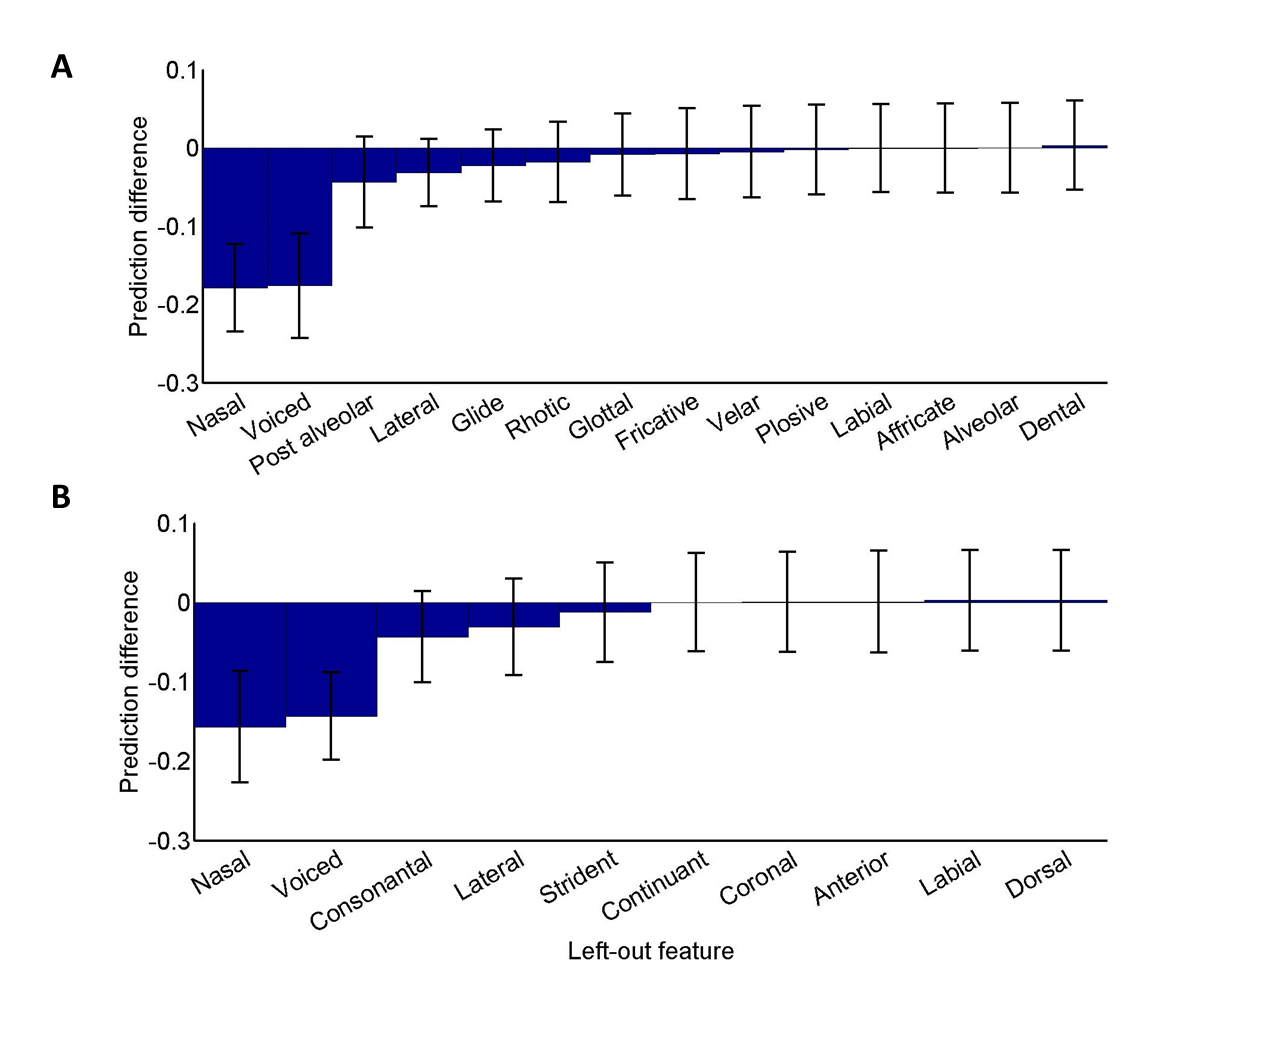
\includegraphics[width=\textwidth]{Figures/Ch2/SWR_prediction.PNG}}
\caption{Reduction in model prediction as a result of omitting a single feature, as calculated for the Luce dataset. (A) Articulatory features (B) Phonological features.}
\end{figure}

%\begin{figure}[H]
%\vspace{.3in}
%\makebox[\textwidth][c]{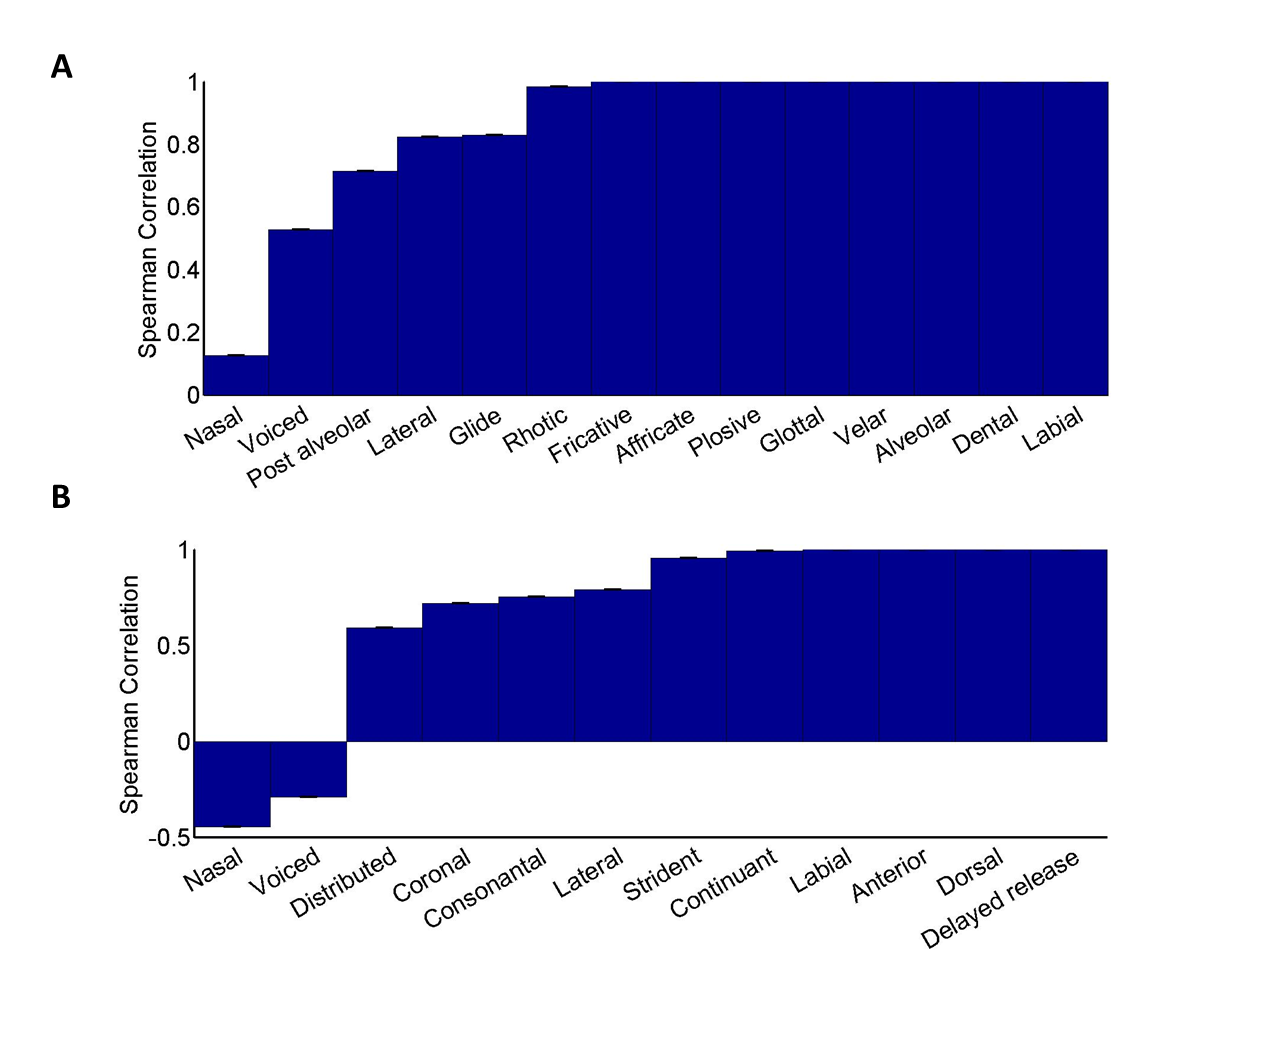
\includegraphics[width=\textwidth]{SWR_corr_Luce.PNG}}
%\caption{Spearman correlation between the weights of the full model and that of a model without a feature. (A) Articulatory features (b) Phonological features.}
%\end{figure}

